\section{Software design} \label{chap:software}
In this section, we first describe the settings used to configure the different modules of the microcontroller and then introduce the controller design 

\vskip 0.2in
\noindent
\textbf{MCU specification:}
\vskip 0.1in
\noindent
As mentioned in the Hardware section, we choose to build the robot using the dsPIC33FJ64MC804 microcontroller since it has two quadrature encoder interface modules and will enable to control both wheels of the motor and provides other features listed below:
\begin{itemize}
    \item 44 pins
    \item 3.3V device 
    \item 16-bit wide data path
    \item up to 40 MIPS operation
    \item Flexible clock options (External, crystal, resonator, internal RC)
    \item Flash program memory (up to 128 Kbytes)
    \item Data SRAM (up to 16 Kbytes)
    \item Peripheral pin Select functionality
    \item Up to 35 programmable digital I/O pins
    \item 2-Quadrature Encoder Interface modules
    \item Peripherals with supported DMA functionality
\end{itemize}
For more details refer to datasheet (pages 3-5)

\subsection{Primary configuration}

\subsubsection*{Configuration bits}

Configuration bits define the microcontroller’s behaviour and enable to set its essential features (Watchdog timer, System Clock Oscillator mode, Phase-Locked Loop, ...).\\
These settings are required before the program starts to run and cannot be changed during the run-time.\\
\vskip 0.1in
\noindent
We invoke pre-processors macros to set the device configuration bits in the main header file.\\
In the main c file, we configure PLL to set the internal clock frequency, call all initialization functions for each of the modules and finally run an infinite background loop so that the system never stops.
\vskip 0.2in
\noindent
\textbf{Oscillator setup}
\vskip 0.1in
\noindent
Configure Phase Lock Loop (PLL) for the system clock reference at 40MHz 
	$$F_{IN} (Oscillator frequency) = 16MHz  $$  
    $$F_{OSC} (Clock frequency) =  80MHz$$
 	$$F_{CY} = 1/2 * F_{OSC} = 1/2 * (F_{IN}*M/(N1*N2)) = 0.5 * (16MHz*20/(2*2)) = 40 MIPS$$
$$Fcy=40Mhz, Tcy=25ns$$
After the PLL setup, we wait in while loop, for PLL to lock, i.e. stabilize. 

\subsubsection*{Pin Mapping}

Peripheral Pin Select (PPS) allows the programmer to map the I/O of most digital peripherals to a selection of pins using an internal switch matrix.
PPS capable pins are identified in the pinout with the designation RPn, with n the port’s pin number. 
\vskip 0.2in
\noindent
\textit{Strategy for pin choice}
\vskip 0.1in
\noindent
We start by selecting fixed pins for the following modules / functions: A2D, PWM, OSCL, Programmer, MCLR. We then, find a pin mapping for the rest of the peripherals from the remappable pins that optimizes the PCB wiring.

\textcolor{red}{
maybe a diagram of which peripheral maps to which pin
}
\vskip 0.2in
\noindent
\textit{Software:}
\vskip 0.1in
\noindent
Before performing pin remapping, we unlock the oscillator, configure the pin mapping, lock the oscillator (enable it again) and wait for a short delay for the remapping to stabilize.\\
The setup differs between input and output pins. For input pin mapping, we need to configure the pin number to the peripheral register. For output pin mapping, we choose the pin register and then map it to the corresponding device code (table 11-2 in datasheet)

\subsection{Peripherals}
\subsubsection*{Timer 1}
The dsPIC33F device family offers several 16-bit Timer modules. We use the timer 1 to function as a real time clock that generate cyclic internal events.\\
We set the timer period to 10ms, which is derived from the external oscillator clock.
$$tick=prescaler*T_{CY}= 64*25ns= 1.6us $$ 
We derive the maximum count with:
$$max\_count=(10 ms)/tick=6250 (6250<2^{16}-1)$$

Hence, we set the period \textbf{PR = 6250 - 1} with a prescaler of \textbf{64}. We choose a high prescaler due to reasons mentioned in \ref{subsec:timer}

\subsubsection*{Pulse Width Modulation (PWM)}

Pulse Width Modulation allows us to control the amount of energy supplied to an actuator. In this case we use the PWM signal to drive our motors and control their speed. Using different pulse widths, we can supply different amount of power to our motors. \cite{alex}
\vskip 0.1in
\noindent
We want to set the registers, such that we achieve a frequency of 20 kHz.
$$f_{PWM} = 20 kHz$$
$$T_{PWM} = \frac{1}{f_{PWM}} = 50 us$$

We fix the prescaler to be \textbf{1}. Given that $T_{PWM} = 50 us$ and $T_{CY}=25 ns$, we conclude:

$$T_{PWM} = prescaler * T_{CY} * (PTPER + 1)$$
$$\iff PTPER = \frac{T_{PWM}}{T_{CY}} - 1  = 2000 - 1 = 1999$$
\vskip 0.1in
\noindent
Depending on our PWM period, we get different amount of ripple in our resulting signal. More on this can be found in \cite[Chapter~5.1]{alex}.
\vskip 0.1in
\noindent
Our PWM duty cycle can take the following values: $PDC \in [0, 2*(P1TPER + 1)] = [0, 4000]$


\subsubsection*{Quadrature Encoder Inferface(QEI)}
To measure the position and velocity of our motors, we are provided with a \textit{quadrature encoder}.
The following values are set twice for each motor (left and right).
\vskip 0.1in
\noindent
Our motor from the Faulhaber 2619 series posesses 16 lines per revolution. If we were to measure only the amount of times light is registered on the photo-transistors, the maximum counts for one revolution would be 16. But since we can also count the times it turns off, we can go up to 32 measurements per revolution. Lastly taking the two channels, A and B, into consideration, we get 64 counts per revolution.
\vskip 0.1in
\noindent
We call this setting \textbf{edge gain}. In our case we have set it to 4 to achieve 64 counts per revolution.
\vskip 0.1in
\noindent
Our $POSCNT$ stores the current position of our wheel and our $MAXCNT$ register stores the maximum value we count to.
\vskip 0.1in
\noindent
We set $MAXCNT$ to the maximum possible value \textbf{0xffff} and $POSCNT$ to half of it.


\subsubsection*{Analogue-to-Digital Conversion(ADC)}

To convert the analogue sensor values to digital values that can be processed by the controller, we configure the ADC module. \\
We sample 3 analogue channels for our 3 sensors: AN4, AN6, AN8 using a configuration with 12-bit conversion (output is an unsigned integer) and 1 sample and hold unit.
\vskip 0.1in
\noindent
In a general configuration, ADC raises an interrupt when all the configured channels have been sampled and the results are available on the 16-bit ADC buffers but Since our device has a DMA module, the storing of converted values can be automated without the need of CPU involvement and disable the ADC interrupt.
\vskip 0.1in
\noindent
\textbf{Sampling and conversion settings:}
\vskip 0.1in
\noindent
Requirements from datasheet table 31-16: 
\begin{itemize}
    \item minimum conversion clock $T_{AD} = 117.6 ns$
    \item minimum acquisition time $T_{ACQ}=3*tad= 352.8ns $
    \item maximum sampling rate for 12 bit conversion is 500 Ksps
\end{itemize}
\vskip 0.1in
\noindent
We derive the ADC Conversion Clock from the system clock with:
\begin{itemize}
    \item Conversion clock: $T_{AD}=T_{CY}*(ADCS+1)= T_{CY}*8 = 8/40M= 200ns (200ns>117.6ns)$
    \item Acquisition time: $T_{ACQ}= SAMC*T_{AD}= 5*T_{AD}=1us (1us>352.8ns)$
    \item ADC total Conversion time (12 bit): $T_{CONV}=14*T_{AD}=2.8us$
    \item sampling rate (user 10ms timer) is 100sps ($100sps < 500Ksps$)
\end{itemize}
$$T_{SAMP}-(T_{ACQ}+T_{CONV})*3=10ms-6us$$ 
Hence, we have enough margin since the sampling starts not immediately after last conversion but when ASAM bit is set in timer ISR.
\vskip 0.2in
\noindent
\textbf{Remarks:}
\vskip 0.1in
\noindent
If the acquisition time is too short, the sample and hold will not settle and the accuracy will decrease.\\
During the conversion the capacitor is discharging. If the conversion time is too long, we lose accuracy. \\
We tried to find a trade-off between to ensure optimal accuracy.

\subsubsection*{Direct Memory Access (DMA)}

We define a DMA data buffer adcData, a global variable where all conversion results are stored in the same order in which the conversions are performed by the ADC module.\\
We store one sample per channel and generate an interrupt after the 3 channel values have been transferred. The interrupt service routine stops the sampling that is again started at each timer interrupt call. 
\vskip 0.1in
\noindent
We set the dma operating mode to a peripheral indirect addressing mode ((peripheral generates destination address [increment by 2]) and a continuous no ping pong setting (continuous transfer of data with the same buffer start address) as shown in the figure below:

\begin{figure}[H]
    \centering
    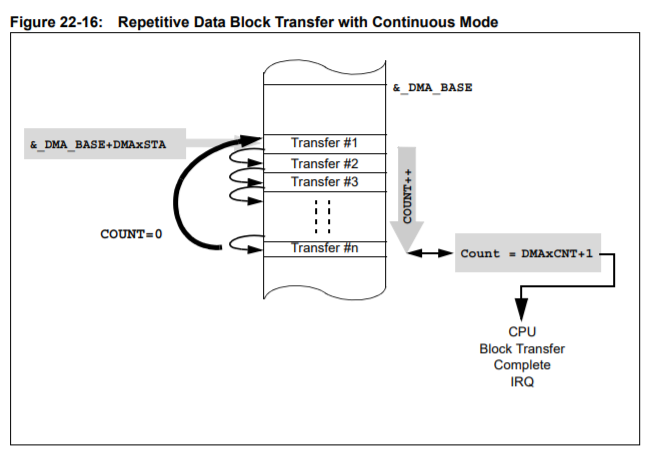
\includegraphics[width=0.5\textwidth]{figures/software/DMA.png}
    \caption{DMA continuous no ping pong mode}
    \label{fig:dma}
\end{figure}

\subsubsection*{Universal Asynchronous Receiver Transmitter (UART)}
Our dsPIC33FJ64MC804 has a Universal Asynchronous Receiver Transmitter (UART)  module for serial port communication.
The UART can communicate with peripheral devices. 
In our case, we use it to commmunicate with an outside computer to send commands or read out values. This was especially useful to find fitting parameters for our gains in the controller logic (chapter).

\begin{figure}[htb]
    \centering
    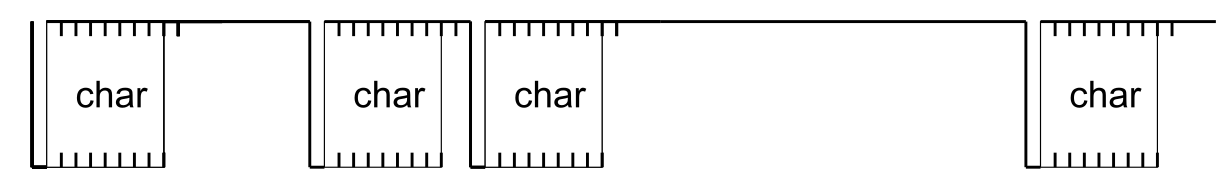
\includegraphics[width=0.6\textwidth]{figures/software/uart_demo.png}
    \caption {String transmission of 8 bit characters with one start bit and one stop bit (no parity) \cite{alex}}
    \label{fig:uart_demo}
\end{figure}

Figure \ref{fig:uart_demo} shows the transmission of a string consisting of three characters. 
The dsPIC33FJ64MC804 allows us to specify the properties of our transmission. The most important settings:
\begin{itemize}
    \item Baud rate: 57.6 kbit/s
    \item Data Selection Bits: 8
    \item Parity bit: 0
    \item Stop bit: 1
\end{itemize}

In order to send out messages, we require another module. We therefore connect our microcontroller to the \textbf{HC-05 Bluetooth Module} (figure \ref{fig:hc_05} so that we can send messages to that module which again transfers those messages via bluetooth to our computer where we read out the values.

\begin{figure}[htb]
    \centering
    \begin{minipage}{.5\textwidth}
          \centering
            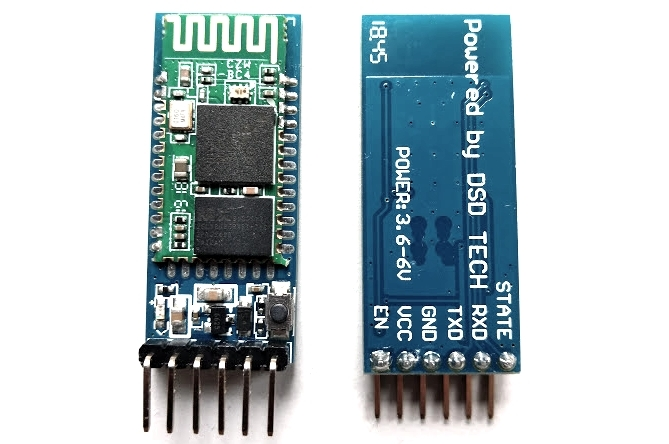
\includegraphics[width=.9\linewidth]{figures/software/uart_hc05.jpg}
              \caption{HC-05 Bluetooth Module}
                \label{fig:hc_05}
    \end{minipage}%
    \begin{minipage}{.5\textwidth}
          \centering
            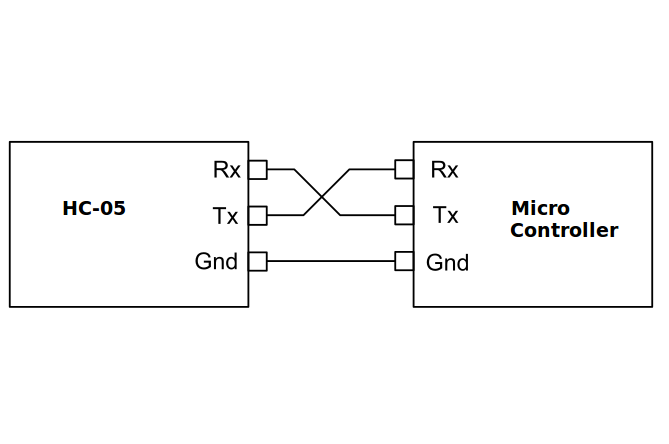
\includegraphics[width=.9\linewidth]{figures/software/uart_plug.png}
              \caption{Connecting the HC-05 module to our microcontroller}
                \label{fig:wire_3}
    \end{minipage}
\end{figure}

The 3-wire UART as seen in figure \ref{fig:wire_3} shows our configuration for a full-duplex communication. The Bluetooth module sends out the message it gets on the reception line (Rx) and sends back messages to the microcontroller through its transmission line (Tx). To receive the message from our microcontroller, we need to connect our computer to the HC-05 module via bluetooth.

It is important to configure the baud rate of the HC-05 module in advance, such that it matches our microcontroller's baud rate. Also, in order to read out values, the baud rate on the PC we are reading from, must also match (in this case 57.6 kbit/s)


\subsection{Controller Design and Approach}

\textcolor{red}{
Here goes the whole logic of the mouse movement control (how should it behave when is faced with the wall or on contrary - with the gap in the labyrinth). PID controller design and the logic behind it.
}

\subsubsection{Proportional-Integral-Derivative Controller (PID)}
\subsubsection*{Need for control loop feedback}

The robot velocity is controlled by varying the PWM duty cycle but it is not guaranteed that the motor is driving exactly at this value. A feedback mechanism is necessary to control and verify this value.\\
\vskip 0.1in
\noindent
A proportional–integral–derivative controller (PID) is a control loop feedback mechanism widely used in industrial control systems and a variety of other applications requiring continuously modulated control. A PID controller continuously calculates an error value e(t) as the difference between a desired setpoint (SP) and a measured process variable (PV) and applies a correction based on proportional, integral, and derivative terms.\\
The overall control function can be expressed mathematically as : 
$$Output = K_{P}*e(t) + K_{I}*\int_t e(t) dt + K_{d}*\frac{d e(t)}{dt} $$
$$e(t) = setpoint - input $$
\noindent
where Kp, Ki, and Kd, all non-negative, denote the coefficients for the proportional, integral, and derivative terms respectively.

\subsubsection*{P term}

KP is proportional to the current value of the error. \\
A simple P controller prevents the system from reaching its target value. The system settles in a steady state error since it requires an error to generate the proportional response.\\
\vskip 0.1in
\noindent
\textcolor{red}{add graph here}
Graph test1 : Test of P controller on the motor. the target value is not reached
\subsubsection*{I term}

It accounts for past values of the error and integrates them over time to produce the I term. \\
Introducing the I term, solves the previous problem with a historic cumulative value of the error.
\vskip 0.1in
\noindent
\textcolor{red}{add graph here}
Graph test 2: Test of PI controller on the motor. The target value is reached

\subsubsection*{Clamping I term and PID output}

The integral term can grow very largely through time, especially when the set point cannot be reached and may lead to a saturating the output or inducing a lag of the response in the step down, i.e. when decreasing the setpoint. For this reason, it’s necessary to limit this term.\\
Since the controller registers have a limit, it is also necessary to limit the output of the controller for sanity check. 

\subsubsection*{Cascade controller: position and velocity}

We use two controllers to adjust both the position and speed of each wheel. 
\vskip 0.1in
\noindent
The position control is performed with a simple P controller which error is the different between the measures distance to the wall of the right and left sensors. The goal is to have the robot in the middle of the cell, i.e. with the same distance to the right and left wall.\\
We only need a P controller because the inertia of the robot leads to an integration (the wheels automatically integrate) as the robot moves on.
\vskip 0.1in
\noindent
The output of this controller (desired velocity) is used as the setpoint for the PI controller that adjusts the speed of the wheel. It takes as input the error between the desired and current velocity and returns a PDC value that sets the new motor speed.
\vskip 0.1in
\noindent
To find the optimal parameters that maximize the responsiveness to the error we perform loop tuning. Refer to test section for more on loop tuning. 

\subsubsection{State Machine}



